\begin{figure}[H]\centering
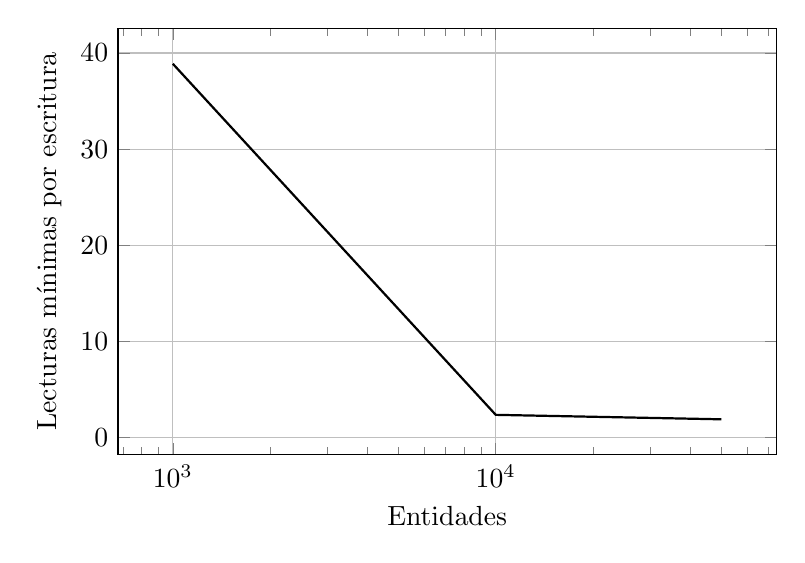
\begin{tikzpicture}\begin{axis}[width=.82\textwidth,height=7cm,xmode=log,log basis x=10,xlabel={Entidades},ylabel={Lecturas mínimas por escritura},grid=major,mark=*]
\addplot[black,thick] coordinates {(1000,38.87477) (10000,2.37132) (50000,1.90685)};\end{axis}\end{tikzpicture}
\caption{Umbral temporal para justificar C1 frente a B1 en el perfil R.}\label{fig:equilibrio-fase3}\end{figure}
